
\documentclass[twoside,twocolumn]{article}
\usepackage{datetime}
\usepackage{blindtext,qtree,amsmath} % Package to generate dummy text throughout this template 
\usepackage{graphicx,floatrow}
\usepackage{algorithm}
\usepackage{algorithmic}
\usepackage[sc]{mathpazo} % Use the Palatino font
\usepackage[T1]{fontenc} % Use 8-bit encoding that has 256 glyphs
\linespread{1.05} % Line spacing - Palatino needs more space between lines
\usepackage{microtype} % Slightly tweak font spacing for aesthetics

\usepackage[english]{babel} % Language hyphenation and typographical rules

\usepackage[hmarginratio=1:1,top=32mm,columnsep=20pt]{geometry} % Document margins
\usepackage[hang, small,labelfont=bf,up,textfont=it,up]{caption} % Custom captions under/above floats in tables or figures
\usepackage{booktabs} % Horizontal rules in tables

\usepackage{lettrine} % The lettrine is the first enlarged letter at the beginning of the text

\usepackage{enumitem} % Customized lists
\setlist[itemize]{noitemsep} % Make itemize lists more compact

\usepackage{abstract} % Allows abstract customization
\renewcommand{\abstractnamefont}{\normalfont\bfseries} % Set the "Abstract" text to bold
\renewcommand{\abstracttextfont}{\normalfont\small\itshape} % Set the abstract itself to small italic text

\usepackage{titlesec} % Allows customization of titles
\renewcommand\thesection{\Roman{section}} % Roman numerals for the sections
\renewcommand\thesubsection{\roman{subsection}} % roman numerals for subsections
\titleformat{\section}[block]{\large\scshape\centering}{\thesection.}{1em}{} % Change the look of the section titles
\titleformat{\subsection}[block]{\large}{\thesubsection.}{1em}{} % Change the look of the section titles

\usepackage{fancyhdr} % Headers and footers
\pagestyle{fancy} % All pages have headers and footers
\fancyhead{} % Blank out the default header
\fancyfoot{} % Blank out the default footer
%\fancyhead[C]{Running title $\bullet$ May 2016 $\bullet$ Vol. XXI, No. 1} % Custom header text
\fancyfoot[RO,LE]{\thepage} % Custom footer text

\usepackage{titling} % Customizing the title section
\usepackage{listings}
\usepackage{hyperref} % For hyperlinks in the PDF

%----------------------------------------------------------------------------------------
%	TITLE SECTION
%----------------------------------------------------------------------------------------

\setlength{\droptitle}{-4\baselineskip} % Move the title up

\pretitle{\begin{center}\Huge\bfseries} % Article title formatting
\posttitle{\end{center}} % Article title closing formatting
\title{Implementing MAXQ and Qlearning methods in R and applying them to the taxi problem \thanks{Reinforcement learning undergraduate class project}}% Article title
\author{%
\textsc{Mihai Groza} \\[1ex] % Your name
\normalsize Concordia University \\ % Your institution
\normalsize \href{mailto:fill this}{fill this} % Your email address
\and % Uncomment if 2 authors are required, duplicate these 4 lines if more
\textsc{Khaled Fouda} \\[1ex] % Second author's name
\normalsize Concordia University \\ % Second author's institution
\normalsize \href{mailto:khaledsfouda@gmail.com}{khaledsfouda@gmail.com} % Second author's email address
}

%\newdate{date}{02}{02}{2020}
%\date{\displaydate{date}}
%\date{\today} % Leave empty to omit a date
\renewcommand{\maketitlehookd}{%
\begin{abstract}
last thing to do.
\end{abstract}
}

%----------------------------------------------------------------------------------------

\begin{document}

% Print the title
\maketitle

%----------------------------------------------------------------------------------------
%	ARTICLE CONTENTS
%----------------------------------------------------------------------------------------

\section{Introduction}
later.
%------------------------------------------------
\section{Environment}
%\begin{center}
\begin{figure}
\centering
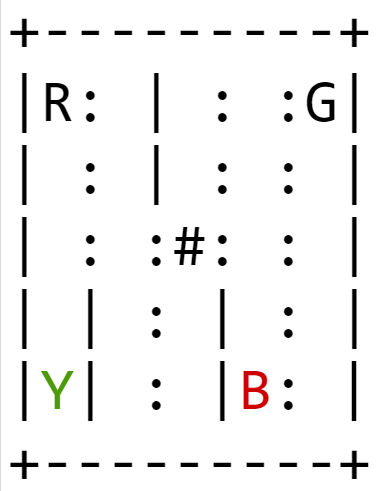
\includegraphics[scale=.4]{taxi.png} 
\caption{generated by render(s)}
\end{figure}
%\end{center}
The taxi's - shown as \# - goal is to first pick up the passenger from one of the four places (R,Y,G,B) where the current location of the passenger is shown in green. After picking up the customer, the next and final goal is to drive him to his destination which is one of the four places (R,Y,G,B) and the destination is shown in red.\\

The state is defined as a set (taxi\_row, taxi\_column, passenger\_location, destination\_location) where:\\
taxi\_row and taxi\_column take values from 1 to 5 as we have 5x5 grid,\\
passenger\_location and destination\_location take values [1,2,3,4] for [R,Y,G,B], furthermore, if the passenger is in the taxi then they takes a location 5.\\
That being said, we have $5*5*5*4=500$  different states.\\

The set of actions available is ( North, South, East, Wast ) with ids 1 to 6.\\

If the taxi successfully dropped off the passenger then the episode is over and they receive a reward of +20, if they dropped the passenger at a wrong location or before picking them up first then they receive a reward of -10 and continue the episode to drop the passenger at the right location (ie. no change in the state). Similarly if they attempted to pick the passenger at the wrong place. Otherwise, they receive a reward of -1 for each step taken. Note that hitting the wall results in a reward of -1 and no change in the state.\\

I have implemented the following functions for the environment:\\
\begin{itemize}
\item render(state) : returns nothing and prints out the environment at the current state.\\

\item encode(s) : maps each state to an integer between 1 and 500.\\

\item decode(i): The inverse of encode(s). it takes an integer between 1 and 500 and returns the corresponding state.\\

\item loc.indx(i): maps the four pick/drop locations (1,2,3,4) to a (row,column) set.\\

\item hitting.wallQ(r,c,a): returns True if taking the action (a) at the location (r,c) would results in hitting the wall.\\

\item step(s,a) returns (s',r) at state s, it takes the action a, observes the reward r and the next state s' 
\end{itemize}
 
%-------------------------------------------------
\section{MAXQ method}
In our problem, the agent's goal is not only reaching the destination but is to also pick up the customer first. From this we define the following sequence of subtasks needed to reach the goal. \\

\textbf{Reach the customer $\Rightarrow$ Pick them up $\Rightarrow$ Drive to the destination $\Rightarrow$ drop them off} \\

MAXQ algorithm is one  of the hierarchical reinforcement learning methods which guarantees ultimate goal satisfaction only if a sequence of sub-goals was satisfied. \\
One the other hand, the algorithm's performance depends on how the structure of hierarchy is defined. MAXQ0 provides no way of learning that structure.\\
In MAXQ there are two types of actions: a primitive action which is the action that change the state of the environment and composite action which is a sub-task. For our Implementations, we defined the following actions:
\begin{itemize}
\item Primitive actions:
\begin{enumerate}
  \item Move one step north (N)
  \item Move one step south (S)
  \item Move one step east (E)
  \item Move one step south (W)
  \item pick-up the passenger
  \item drop-off the passenger
\end{enumerate}
\item subtasks actions:
\begin{enumerate}
  \setcounter{enumi}{6}
  \item Root - explained below -
  \item reach the customer and pick them up (GET)
  \item drive to the destination and drop them off (PUT)
  \item drive to the customer (Navigate\_C)  
  \item drive to the destination (Navigate\_D)
\end{enumerate}
\end{itemize}
and Their hierarchical structure is defined as follows:
\begin{center}
\Tree[.Root 
		[.GET  [.Pick ] [.Navigate\_C N S E W ] ]
        [.PUT  [.Navigate\_D N S E W ] [.Drop ] ] ]

\end{center} 
Where - starting at root - the agent has to recursively go down the graph satisfying each composite action. The root is satisfied if both get and put are satisfied and hence the episode ends. At each subtask i, the agent needs to repeatedly choose an action until the task is completed and hence we go back to the parent subtask. \\
For each action, a list of Terminal states is defined. If an action is at a terminal state, it no longer needs move down the tree and it returns back to it's parent subtask. For example, at Navigate\_C, it repeatedly choose one of the four actions [N,S,E,W] until it reaches the location of the customer. When that happens, we say that Navigate\_C reached a terminal state and it stops executing it's subtask and it reports back to it's parent "GET" who either choose an action "Pick" or "Navigate\_C" or if it's at a terminal state, it reports back to root and so on. The only terminal state for root is when both "GET" and "PUT" reached their terminal states and the episode is over.  

\subsection*{value function Estimates}

Let $(i,s)$ define the state of the environment at time $t$ where $i$ is the subtask running. Let also $a$ be the action (sub-subtask) taken by subtask i at time t.
Define 
$$ C^\pi(i,s,a) = (1-\alpha)C^\pi(i,s,a) + \alpha*\gamma^N * V[i,s'] $$
\[
    V^\pi(i,s) =
    \begin{cases}
        (1-\alpha)*V^\pi(i,s) + \alpha * Reward(s'|s,i) &\\ \text{if i is primitive}\\
        max_{a\in A(i)} V^\pi(a,s) + C^\pi(i,s,a) &\\ \text{if i is a subtask}
    \end{cases}
\]\\

where $\alpha$ is the learning rate, $\gamma$ is the discounting factor, $N$ is the number of times the subtask i  executed actions before reaching the terminal state, and $A(i)$ is the set of available actions to  subtask i. \\
$C^\pi$ is only defined for composite actions, i.e, for $i\in (7,8,9,10)$ and it's similar to the usual action value function $Q$ and it it takes into account the value function of the next state produced by a primitive action. the term $\gamma^N$ is adapted from Semi-Markov decision model and it helps prioritizing the actions that leads to smaller number of steps. However, in our experiment, we got better results setting this term 1.\\
The state value function for the primitive actions is a classic weighted average of rewards and for the composite actions is a maximization of a modified action value function.
The state value function for the composite actions requires recursive calculations of the subsequent actions chosen. 
\begin{lstlisting}[language=R]
EvaluateMaxNode <- function(i, s){
  # if i is primitive then do nothing
  if(any(i==1:6)){return()}
  actions <- Action.space(i)
  for(a in actions){ 
	  EvaluateMaxNode(a, s)
  }
  V[i,encode(s)] <- max(V[actions,encode(s)] + 
  C[[i]][encode(s),actions])
}
\end{lstlisting}

\subsection*{Policy}

The policy used is $\epsilon-greedy$. Only composite actions -subtasks- can take subsequent actions and it's the action the maximizes the modified action value function above with probability $1-\epsilon$ and a random action with probability $\epsilon$ with the restriction of belonging to the action space -defined below- of that subtask. 


\subsection*{Action Space}
The action space for each action is the set of sub-nodes related to that action. Remember that only subtasks have action spaces since states with primitive actions take a pre-determined actions defined by the environment above.
\begin{lstlisting}[language=R]
Action.space <- function(.,i){
  # expects i to be from 7 to 13
  if(i==7){return(c(8,9))
  }else if(i==8){return(c(5,10))
  }else if(i==9){return(c(6,11))
  }else if(i==10 || i==11){return(1:4)}
}
\end{lstlisting}

\subsection*{Terminal States}
Each subtask -subtree- runs recursively until it hits one of its terminal states. Terminal states do not necessarily represent the completion of that subtask, they can be states where the subtask is not needed at that time step.
We defined the following terminal states:
\begin{itemize}
\item When either the subtask Get or Navigate\_C is active and the customer being already picked up.
\item When either the subtask Put or Navigate\_D is active and the customer is not yet picked.
\item When either of the navigation subtasks is active and the taxi has already arrived the destination.
\item When the episode is over and the customer have made their trip successfully. 
\end{itemize}
As for the primitive actions, they are always executed once and report back to their parent-node who then can make choice of whether it execute them again using the defined policy.

\subsection*{Learning Algorithm}
\begin{algorithm}
\caption{MAXQ0(node i, state s) }
\begin{algorithmic}[1]
\IF {i is a primitive action}
\STATE execute the pair $(i,s)$ and observe the resulting $(i,s')$
\STATE  $V(i,s) \leftarrow (1-\alpha)*V(i,s) + \alpha * r$
\STATE  $return(1)$
\ELSE
\STATE $count \leftarrow 0$ 
\WHILE{(i,s) not a terminal state}
\STATE choose a according to the policy
\STATE $N \leftarrow MAXQ0(a,s)$
\IF {episode is done}
\STATE $return(count)$
\ENDIF
\STATE $EvaluateMaxNode(i,s)$
\STATE $C(i,s,a) \leftarrow (1-\alpha)C(i,s,a) + \alpha*\gamma^N * V[i,s']$
\STATE $count \leftarrow count + N$
\STATE $s \leftarrow s'$
\ENDWHILE
\ENDIF
\end{algorithmic}
\end{algorithm}
The last function when called with an initial $i=7$-Root- it simulates a full episode from the beginning until the successful drop off of the passenger. For larger scale problems and poorer design of the environment, the while loop might run forever before reaching a terminal state.  


%------------------------------------------------
\section{Qlearning method}
\section{Results}
MAXQ has 4 parameters to tune. The learning rate $\alpha$, the discounting rate $\gamma$, the policy\'s $\epsilon$ and the number of simulated episodes.\\
After many trials, I have chosen the following parameters: $\alpha=.8, \gamma=.999, \epsilon=.01, n=2000$. For $\alpha$ to be that high means we put more weight on newer episodes than old ones. Although in theory that should give better results, in our experiment, $\alpha$'s best value is .8. Here below is a plot showing the evolution of rewards overtime and comparing the model with two different values of $\alpha$. It is clear that the higher $\alpha$ achieved higher rewards.\\
 
\begin{figure}[hbtp]
\centering
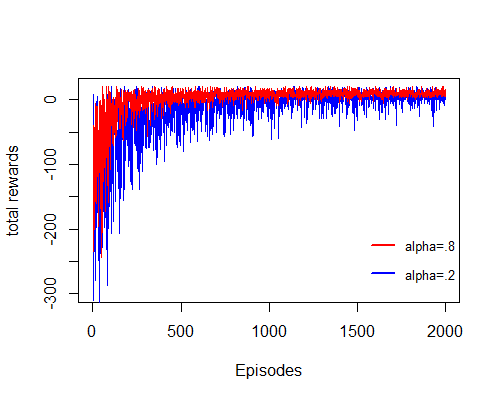
\includegraphics[scale=.8]{RplotHL2.png}
\caption{..}
\end{figure}
Another note is the value of $\gamma$. The models performs well with gamma is 1 compared to values like $.9$ or $.8$. However, I chose the value $.999$ to filter out actions that requires very high number of steps. For example if the agent took 1000 steps to navigate to the destination, then $.999^{1000}=.367$ would give that action a lower value estimate.\\
Finally, I have looked at the statistical summaries \\

\begin{tabular}{c|c|c|c|c}
 min & median & mean & max & variance \\
 \hline
 -244 & 9 & 3 & 20 & 585.8
 \end{tabular} \\
and from the first glance we notice the high variance. However, as in the plot above, for the first 500 episodes the rewards fluctuate a lot and therefore, lets consider only the values starting from episode number 500.\\

\begin{tabular}{c|c|c|c|c}
 min & median & mean & max & variance \\
 \hline
 -17 & 10 & 9.3 & 20 & 30.7 
 \end{tabular} \\

Although the experiment still exhibits  high variance, it is much lower than the first 500 episodes. Also the proximity between the mean and median shows some kind of stability in the rewards.

\section{Similar projects}
\section{Final thoughts}

%----------------------------------------------------------------------------------------
%	REFERENCE LIST
%----------------------------------------------------------------------------------------

\begin{thebibliography}{99} % Bibliography - this is intentionally simple in this template

\bibitem[Figueredo and Wolf, 2009]{Figueredo:2009dg}
Figueredo, A.~J. and Wolf, P. S.~A. (2009).
\newblock Assortative pairing and life history strategy - a cross-cultural
  study.
\newblock {\em Human Nature}, 20:317--330.
 
\end{thebibliography}

%----------------------------------------------------------------------------------------

\end{document}
